\documentclass{article}

\usepackage{graphicx}

\begin{document}

{\bf Quiz \#1; Tuesday, date: 01/23/2018}

{\bf MATH 53 Multivariable Calculus with Stankova}

{\bf Section \#114; time: 2 -- 3:30 pm}

{\bf GSI name: Kenneth Hung}

{\bf Student name: SOLUTIONS}

\vspace*{0.25in}

\begin{enumerate}
\item Consider the parametric equation for a curve:
\[
x = \sqrt{t - 1}, ~~~~ y = \sqrt{t + 3}.
\]
Eliminate the parameter to find a Cartesian equation of the curve. Sketch the curve and indicate with an arrow the direction in which the curve is traced as the parameter increases.

\vspace*{0.25in}

{\em Solution.} There's not much that can be done with the equations in this form, so try squaring both sides: $x^2 = t - 1$ and $y^2 = t + 3$, so $y^2 - x^2 = 4$. The points therefore lie on a hyperbola, but the restrictions of the parametric equations also mean that $x$ and $y$ must both be non-negative.

\begin{center}
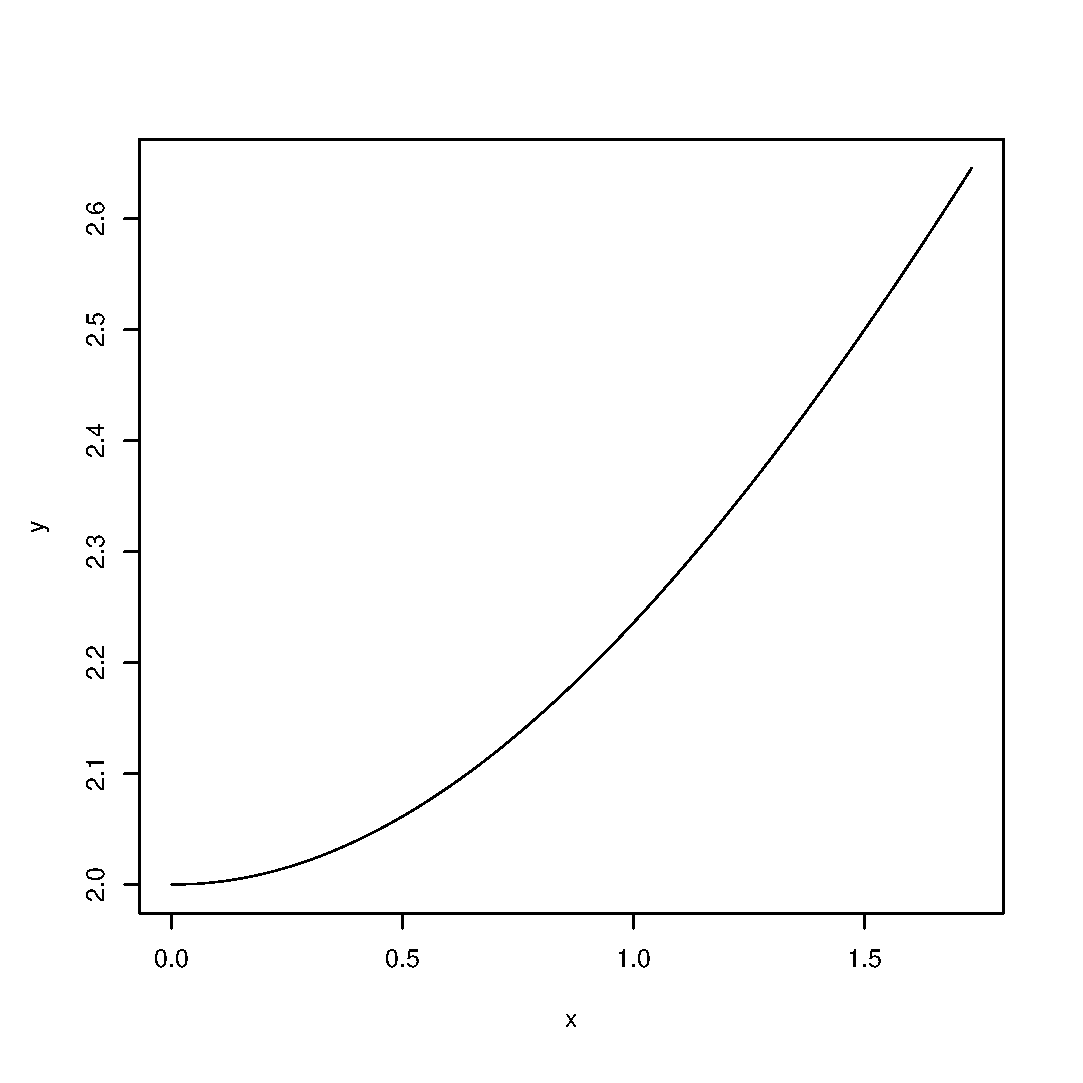
\includegraphics[width=0.8\linewidth]{quiz01dis114solpic.eps}
\end{center}

Both $x$ and $y$ are increasing functions of $t$, but $x$ is defined only when $t \ge 1$. The particle starts at $(0, 2)$ when $t = 1$ and moves upwards (and rightwards) as $t \to \infty$.

\item {\em True / False?} A Cartesian equation $f(x, y) = 0$ of a curve in the plane can always be re-written to define the curve by some function: $y = g(x)$, or by some function: $x = h(y)$.

{\em Solution.} {\bf False}; consider the circle $x^2 + y^2 = 1$. It cannot simply be written as a function as it does not pass the vertical line test.

\item {\em True / False?} The polar curve
\[
r = 2 \cos \theta, ~~~~ 0 \le \theta \le 6 \pi
\]
is a circle centered at $(1, 0)$, traversed $6$ times.

{\em Solution.} {\bf True}; by plugging in some value, one should realize that from $0$ to $\pi$ the circle is traversed once, then proceed to repeat the same path. Since the restriction on $\theta$ is from $0$ to $6 \pi$, the circle is traversed $6$ times.
\end{enumerate}

\end{document}